\subsection*{Задание 1:}
\begin{figure}[H]
	\centering
	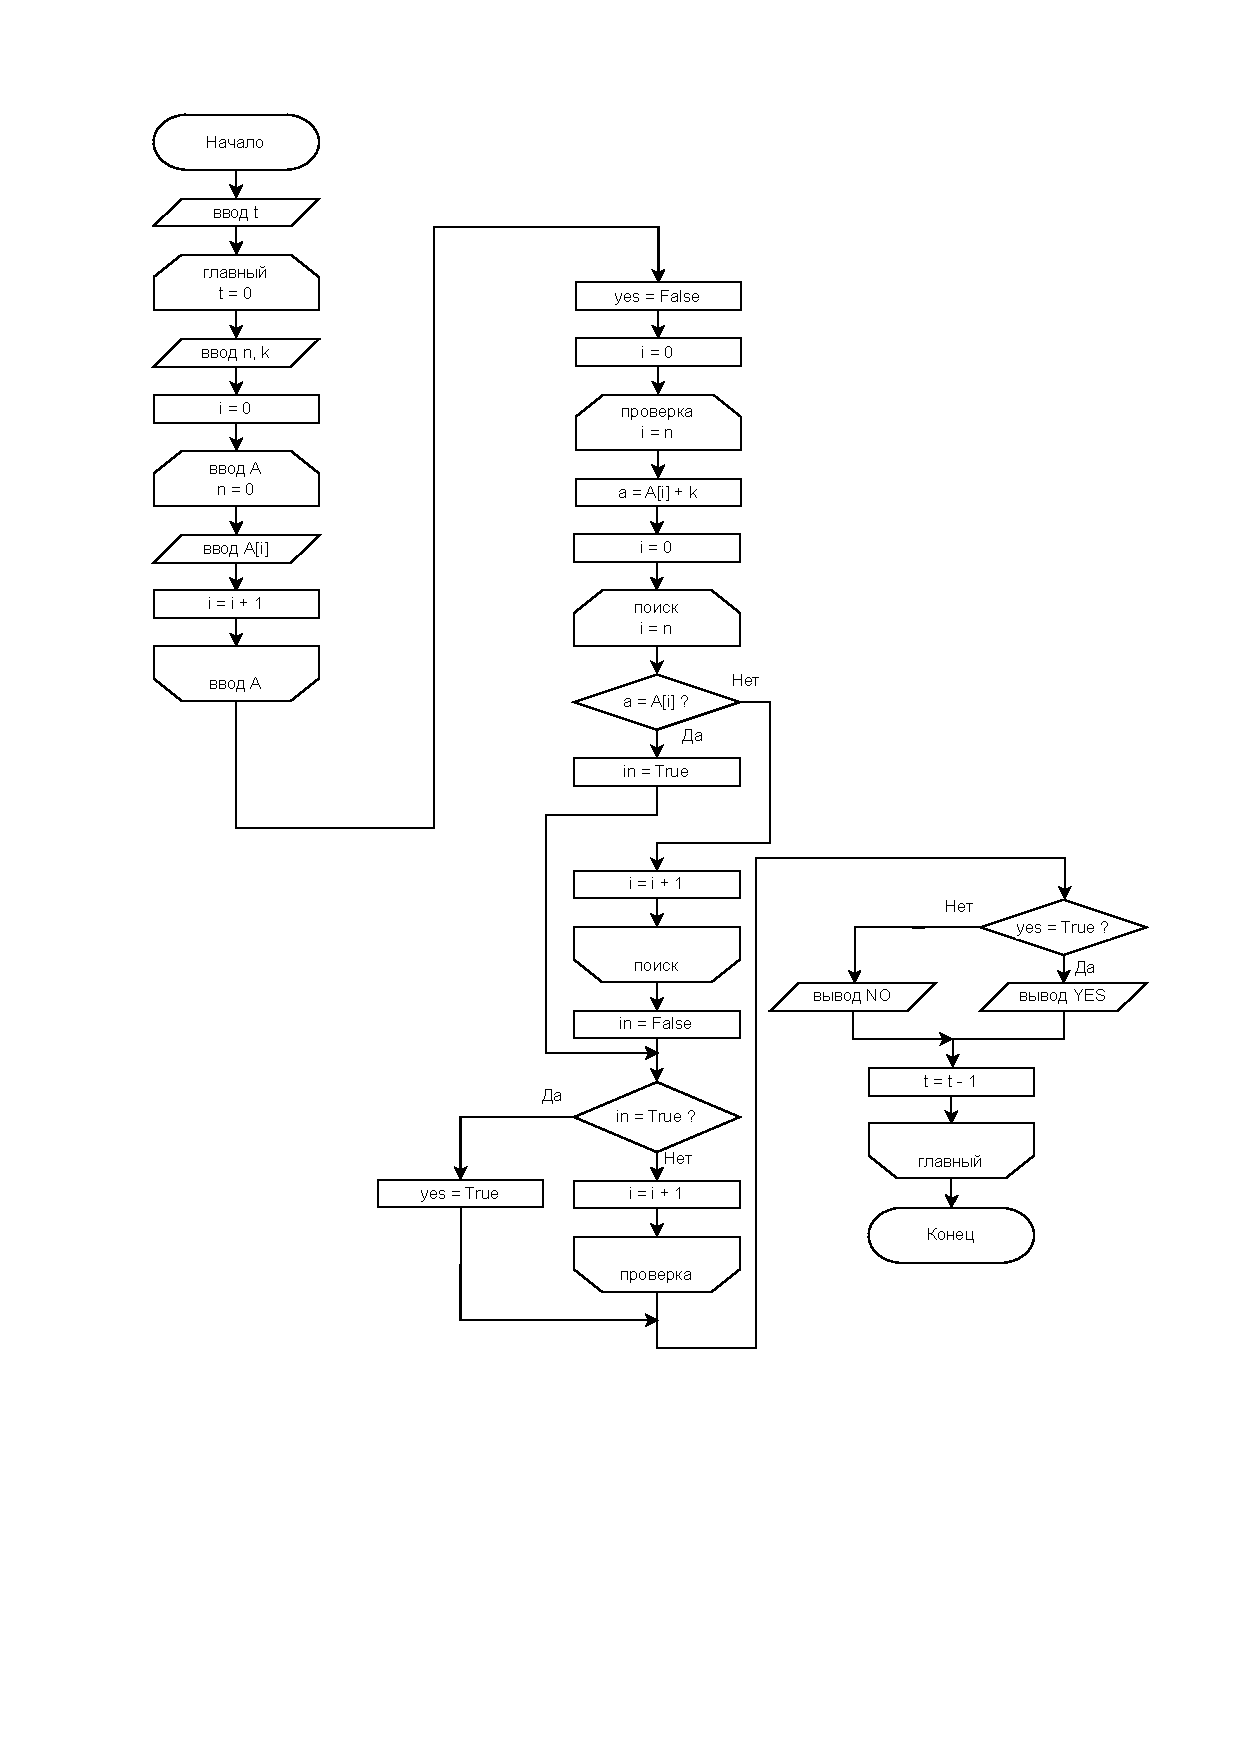
\includegraphics[width=\textwidth, height=0.9\textheight, keepaspectratio]{1.pdf}
	\caption{Схема алгоритма задачи}
\end{figure}
\lstinputlisting[caption={Исходный код программы (Python)}]{1.py}
\noindent \indent

Суть данного задания - проверить, есть ли в исходном массиве 2 числа, разность которых равна k. В коде это реализовано через цикл, 
проходящий по массиву, и сумму текущего числа с k.

\newpage
\subsection*{Задание 2:}
\begin{figure}[H]
	\centering
	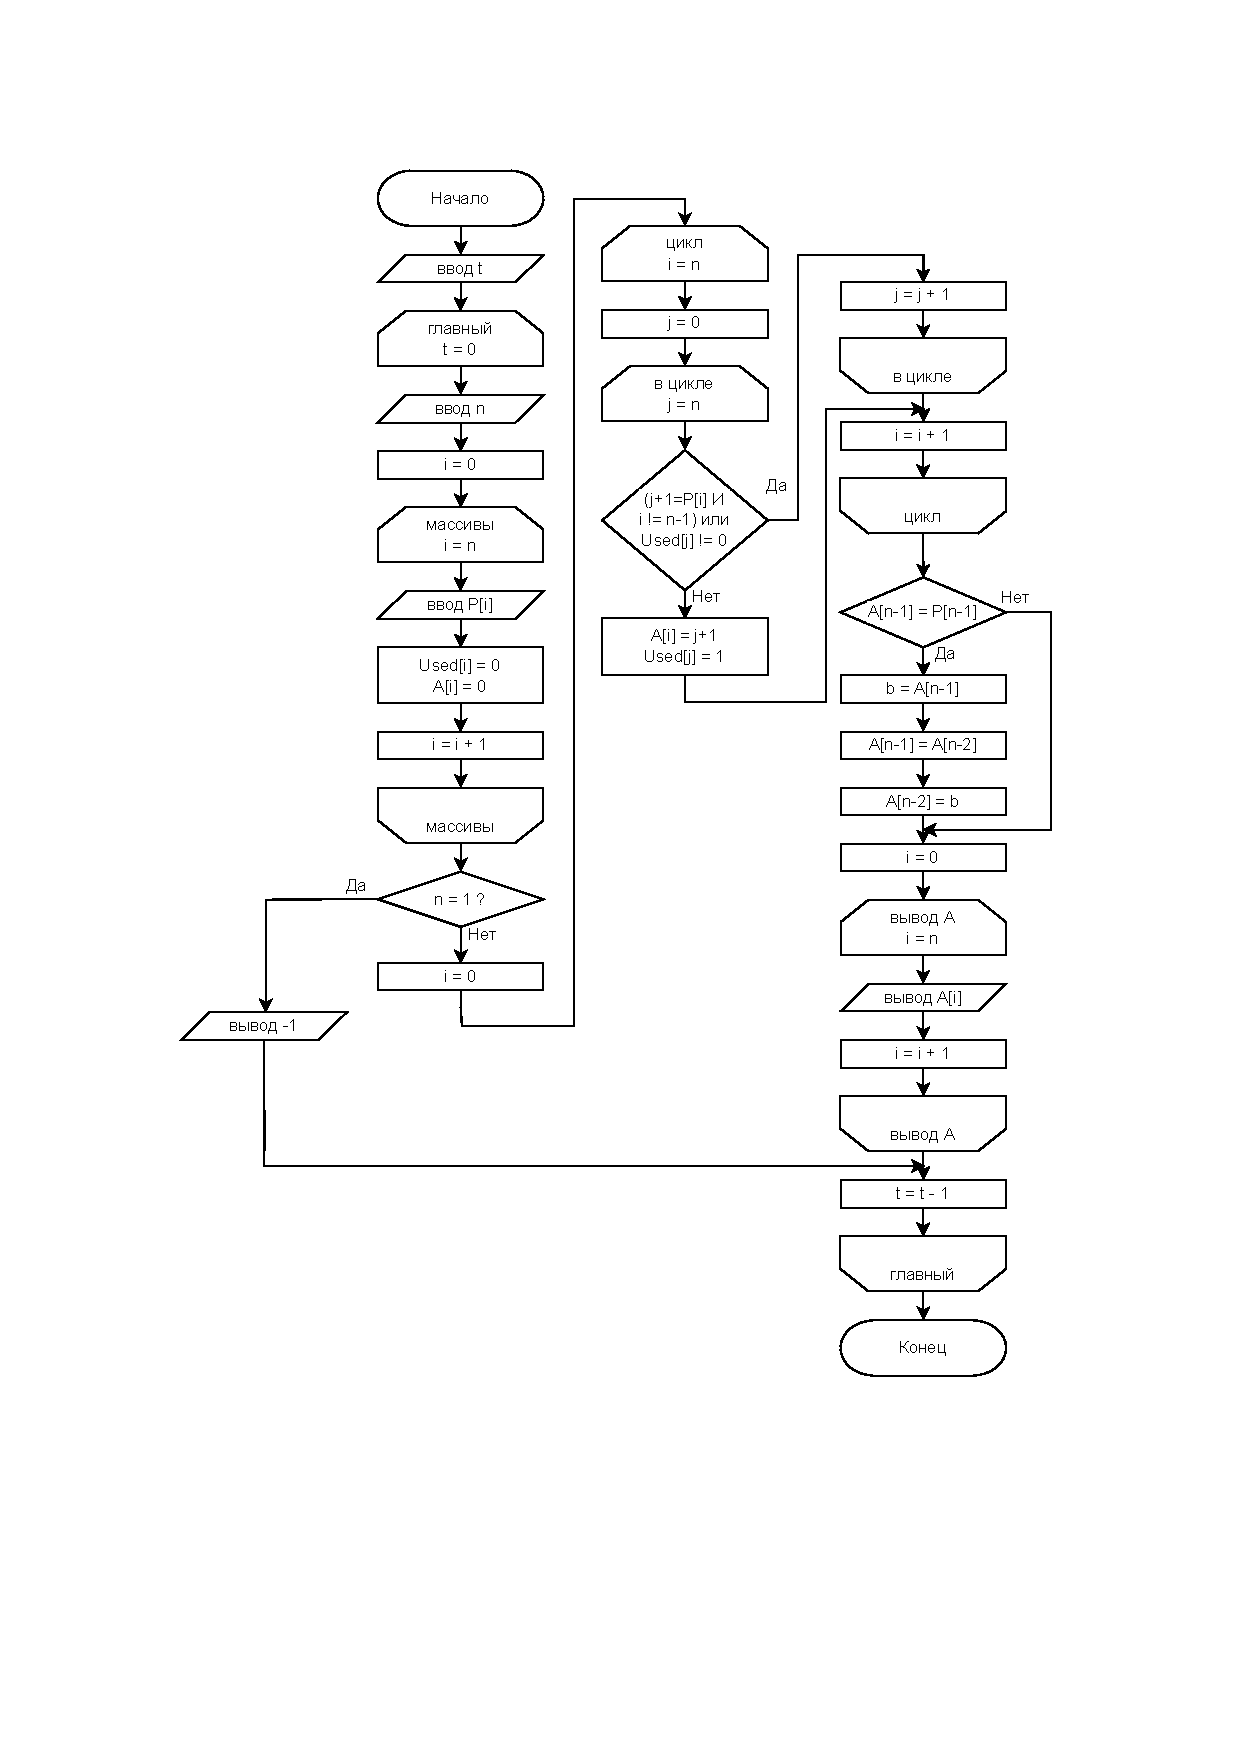
\includegraphics[width=\textwidth, height=0.9\textheight, keepaspectratio]{2.pdf}
	\caption{Схема алгоритма задачи}
\end{figure}
\newpage
\lstinputlisting[caption={Исходный код программы (Python)}]{3.py}
\noindent \indent

Суть данного задания - для каждой позиции пытаться подставить самое маленькое еще не использованное число, не совпадающее с число в этой позиции в исходном массиве.
Если совпадает, берем следующее по величине число. Для последнего числа проверяем, совпадает ли оно с числом из исходного массива - если да, меняем последнее и предпоследнее местами.

\newpage
\subsection*{Задание 3:}
\begin{figure}[H]
	\centering
	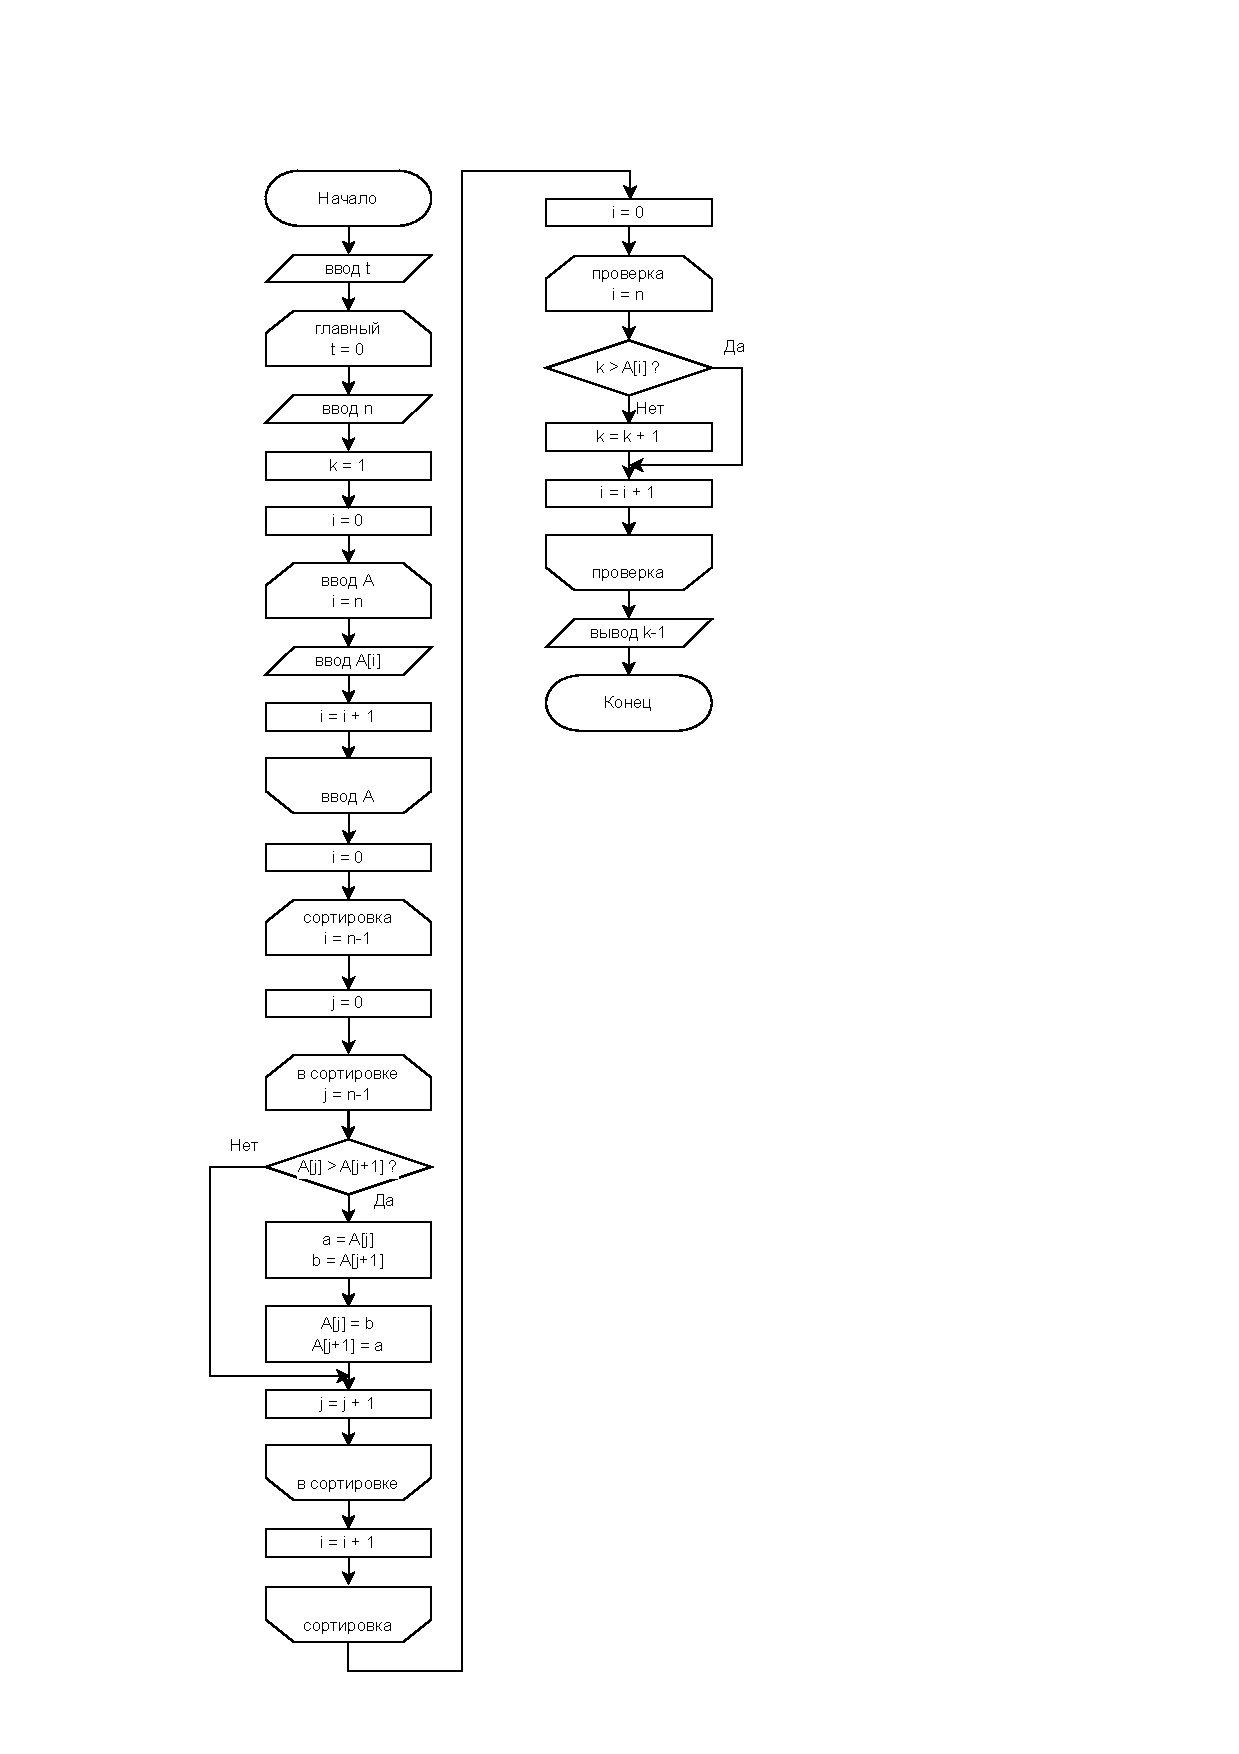
\includegraphics[width=\textwidth, height=0.9\textheight, keepaspectratio]{3.pdf}
	\caption{Схема алгоритма задачи}
\end{figure}
\newpage
\lstinputlisting[caption={Исходный код программы (Python)}]{3.py}
\noindent \indent

Суть данного задания - отсортировать массив по возрастанию и завести счетчик k для определения "текущего" дня по счету. Если в i-ый день кол-во контестов меньше k, пропускаем этот день,
В ином случае - увеличиваем k на 1 (т.е. переходим на следующий день решения контестов).

\newpage